% No subheadings

\section*{Introduction} % 1000 - 1500 words

In recent years, the rapid growth of artificial intelligence (AI) and machine learning (ML) has resulted in increasingly complex and large models in pursuit of higher accuracy and range of use cases~\cite{sevilla22computetrends}.
The substantial growth rate of model computation exceeds efficiency gains realized through Moore and Dennard technology scaling~\cite{shankar22trends}, indicating a looming limit to continued advancements with existing techniques.
This issue is compounded by the open challenges of adapting such methods for resource-constrained edge devices (tinyML) in order to enable pervasive and decentralized intelligence through the Internet of Things (IoT)~\cite{ray22tinyml}.
As such, the urgency for exploring new resource-efficient and scalable computing architectures has intensified.

Neuromorphic computing has emerged as a promising area in addressing these challenges, aiming to unlock key hallmarks of biological intelligence by porting primitives and computational strategies employed in the brain into engineered computing devices and algorithms~\cite{schuman2017survey, james17historical, thakur2018largescale}.
Neuromorphic systems hold a critical position in the investigation of novel architectures, as the brain exemplifies an exceptional model for accomplishing scalable, energy-efficient, and real-time embodied computation.

%% Background %%
Initially, the term ``neuromorphic'' referred specifically to approaches that aimed to emulate the biophysics of the brain by leveraging physical properties of silicon, as proposed by Mead in the 1980's~\cite{Mead:1990hw}. However, the field of neuromorphic computing research has since grown to encompass a wide range of brain-inspired computing techniques at the algorithmic, hardware, and system levels~\cite{schuman2017survey}. 
While the range of approaches is diverse, neuromorphic computing research generally utilizes mechanisms emulating or simulating biophysical properties more closely than conventional methods, aiming to reproduce high-level performance and efficiency characteristics of biological neural systems. 

Neuromorphic \textit{algorithms}~\cite{Schuman2022} encompass neuroscience-inspired methods which strive towards goals of expanded learning capabilities, such as predictive intelligence, data efficiency, and adaptation, and include approaches such as spiking neural networks (SNNs) and primitives of neuron dynamics, plastic synapses, and heterogeneous network architectures.
% Due to the early stages of neuromorphic hardware development, the attributes or scale of neuromorphic algorithms may not yet be adequately supported by existing neuromorphic hardware. As such, current a
Algorithm exploration often makes use of simulated execution on readily-available conventional hardware such as CPUs and GPUs, with the goal of driving design requirements for next-generation neuromorphic hardware. 

Neuromorphic \textit{systems}~\cite{frenkel23bottom} are composed of algorithms deployed to hardware, which seek greater energy efficiency, real-time processing capabilities, and resilience compared to conventional systems. Neuromorphic hardware utilizes a variety of biologically-inspired hardware approaches, including analog neuron emulation, event-based computation, non-von-Neumann architectures, and in-memory processing. Neuromorphic systems target a wide range of applications, from neuroscientific exploration, to low-power edge intelligence and datacenter-scale acceleration.

%% Challenges/Problem statement %%
Despite its promises, progress in the field of neuromorphic research is impeded due to the absence of fair and widely-adopted objective metrics and benchmarks~\cite{Davies19_bencprog, Schuman2022}. Without such benchmarks, the validity of neuromorphic solutions cannot be directly quantified, hindering the research community from measuring technological advancement.
Standard and rigorous benchmarking is necessary for the neuromorphic community to objectively assess and compare the achievements of novel approaches, and make evidence-based decisions on which directions show promise for achieving breakthrough efficiency, speed, and intelligence, thereby helping to focus research and commercialization efforts on techniques that concretely improve on prior work and conventional computing. Neuromorphic benchmarks have been previously proposed for classical vision~\cite{orchard2015converting,Amir_etal17_lowpowe} and audition tasks~\cite{Cramer_2022}, open-loop~\cite{Ostrau2022} and closed-loop~\cite{closedloop-andre} tasks, and for SNN simulator performance assessment~\cite{KULKARNI2021}. While prior works have made valuable contributions, there are opportunities to further advance the field by addressing three outstanding challenges:


\begin{itemize}
    \item \textbf{Lack of a formal definition.} The variety of approaches to exploring brain-inspired principles creates difficulties in defining a set of criteria for what should be benchmarked as a ``neuromorphic” solution. Closed definitions can impose narrow assumptions and thus risk unfairly excluding promising methods.
    This challenge necessitates \textbf{\textit{inclusive}} benchmarks that can be applied generally across the spectrum of potential approaches, allowing for flexible implementation while focusing on task capabilities and metrics of interest such as temporal processing and efficiency.
    Furthermore, the benchmarks should ideally allow for direct comparison of neuromorphic and conventional approaches. 
    
    \item \textbf{Implementation diversity.} A wide array of different frameworks targeting different goals, such as neuroscientific exploration~\cite{nest2007} and automatic SNN training~\cite{eshraghian2021training}, are used in neuromorphic research. This diversity, which has been instrumental in exploring the landscape of bio-inspired techniques following different methodologies and abstraction levels, comes at the cost of portability and standardization, which in turn limits the ease of benchmark implementation. Benchmarks require common infrastructure that unites tooling to enable \textbf{\textit{actionable}} implementation and comparison of new methods.
    
    \item \textbf{Rapid research evolution.} Neuromorphic approaches are continually and rapidly evolving as part of an emerging field. As the research community continues to make technological progress, so too should benchmark suites and methodology expand to foster inclusion and capture salient performance metrics. An \textbf{\textit{iterative}} benchmark framework with structured versioning will facilitate productive foundational and evolving performance evaluation.
\end{itemize}



\begin{figure}[t]
\centering
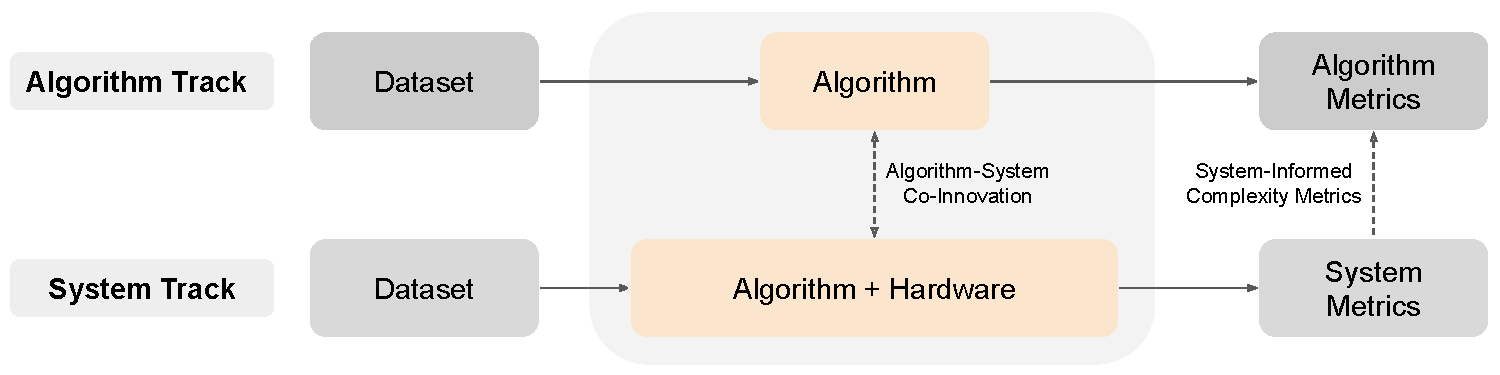
\includegraphics[width=\linewidth]{figures/tracks.pdf}
\caption{The two NeuroBench tracks: algorithms and systems. Grey boxes designate what is defined by the benchmark, and orange boxes indicate what is unique to each solution. Connecting arrows between the two tracks denote the co-innovation between the tracks and the cross-stack innovation enabled by this approach. Between algorithm and system solutions, best-performing results from each track can motivate future solutions to the other. In addition, system metrics and results can inform hardware-independent algorithmic complexity metrics. 
% \note{can augment figure with leaderboard, competition, updating versions over time}
}
\label{fig:tracks}
\end{figure}

To tackle these challenges, this article presents NeuroBench, a dual-track, multi-task benchmark framework. 
NeuroBench addresses the existing neuromorphic benchmark challenges by advancing prior work in three distinct ways. Firstly, the benchmark framework reduces assumptions regarding the specific solution being assessed, encouraging \textit{inclusive} participation of neuromorphic and non-neuromorphic approaches by utilizing general, task-level benchmarking and hierarchical metric definitions which capture key performance indicators of interest. Secondly, the NeuroBench benchmarks are associated with a common open-source benchmark harness tool which facilitates \textit{actionable} benchmark implementation and offers structure for further expansion to neuromorphic algorithm frameworks and systems. Finally, NeuroBench establishes an \textit{iterative}, community-driven initiative designed to evolve over time to ensure representation and relevance to neuromorphic research, analogous to the well-established MLPerf benchmark framework for machine learning~\cite{Reddi2020, mattson2020mlperf}.
As a whole, NeuroBench intends to align the neuromorphic research community on standard benchmarking, providing a dynamically evolving platform to ensure ongoing relevance and facilitate advancements through workshops, competitions, and a centralized leaderboard.

% JY: this should go after the previous paragraph, as the previous is tightly tied to the three points in the list
As Figure~\ref{fig:tracks} shows, the NeuroBench framework involves two tracks to enable agile algorithm and system development. As an emerging technology, neuromorphic hardware has not converged to a single platform which is commercially available, thus a large fraction of neuromorphic research explores algorithmic advancement on conventional systems which may not be optimal for performance. Thus, NeuroBench consists of an \textit{algorithm} track for hardware-independent evaluation and a \textit{system} track for fully deployed solutions. The algorithm track defines four novel benchmarks for neuromorphic methods across diverse domains, namely few-shot continual learning, computer vision, motor cortical decoding, and chaotic forecasting, and utilizes complexity metrics to analyze solution costs. Such hardware-independent benchmarking enables algorithmic exploration and prototyping, especially when simulating algorithm execution on non-neuromorphic platforms. Meanwhile, the system track defines standard protocols to measure the real-world speed and efficiency of neuromorphic hardware on benchmarks ranging from standard machine learning tasks to promising fields for neuromorphic systems, such as optimization. 

Each NeuroBench track includes defined datasets, metric and measurement methodology, and modular evaluation components to enable flexible development. Promising methods identified from the algorithm track will inform system design by highlighting target algorithms for optimization and relevant system workloads for benchmarking. The system track in turn enables optimization and evaluation of performant implementations, providing feedback to refine algorithmic complexity modeling and analysis. The interplay between the tracks creates a virtuous cycle: algorithm innovations guide system implementation, while system-level insights accelerate further algorithmic progress. This approach allows NeuroBench to advance neuromorphic algorithm-system co-design. Both the algorithm and system track will be extended and co-developed as NeuroBench continues to expand.

In the next few sections, we describe the algorithm track, including general complexity metric definitions, benchmark tasks, and common infrastructure tooling. We apply the framework to report baseline results for each algorithm benchmark, which outline unexplored research opportunities in optimizing algorithmic architectures and training of sparse, stateful models to achieve greater performance and resource efficiency. \secondrev{Then, we show baseline results established in the system track to assess neuromorphic performance across promising application workloads.}
By outlining both tracks, we provide a roadmap towards standardizing benchmark procedures in both hardware-independent and hardware dependent settings.

% % This article presents the framework of the NeuroBench benchmark suite. 
% The following Results section organizes descriptions of the algorithm track benchmark framework and its baseline results, as well as specifications of the system track benchmark framework and tasks. Further details regarding the benchmark metric formulations, task specifications, and baseline solutions can be found in the Methods section. Baseline results on NeuroBench benchmarks outline unexplored research opportunities in optimizing algorithmic architectures and training of sparse, stateful models to achieve greater performance and resource efficiency.
% As NeuroBench is intended to continually grow over time, the latest developments and opportunities to engage with the project are reported on the website.\footnote{\href{https://neurobench.ai}{https://neurobench.ai}}
